\section{Sphinx Packet Format}
\label{sec:sphinx}

HOPR uses the Sphinx packet format \cite{sphinxpaper} to encapsulate and route data packets its final recipient while achieving sender and recipient unlinkability. The Sphinx packet format determines how mixnet packets are created and transformed. This happens in a way that does not leak path information to relayers or other parties eavesdropping the communication. A Sphinx packet consists of two parts, a header and an onion-encrypted payload:

\begin{figure}[H]
    \centering
    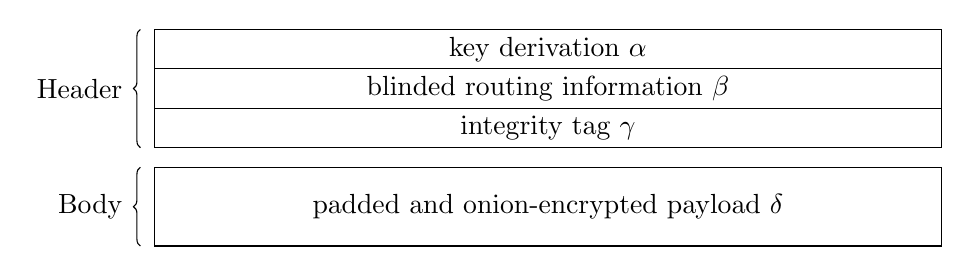
\begin{tikzpicture}
        \draw (0,0) rectangle (10,0.5);
        \draw (0,-0.5) rectangle (10,0);
        \draw (0,-1) rectangle (10,-0.5);

        \draw (5,0.25) node {key derivation $\alpha$};
        \draw (5,-0.25) node {blinded routing information $\beta$};
        \draw (5,-0.75) node {integrity tag $\gamma$};

        \draw[decoration={brace,raise=5pt,mirror},decorate] (0,0.5) -- node[left=8pt] {Header} (0,-1);

        \draw (0,-2.25) rectangle (10, -1.25);
        \draw (5,-1.75) node {padded and onion-encrypted payload  $\delta$};

        \draw[decoration={brace,raise=5pt,mirror},decorate] (0,-1.25) -- node[left=8pt] {Body} (0,-2.25);
    \end{tikzpicture}
    \label{fig:sphinxoverview}
    \caption{Schematic overview of a SPHINX packet}
\end{figure}

\subsection{Construction}

The following explains how a Sphinx packet is created and how it is transformed at each hop before arriving at its final destination. At first, the sender chooses a path (see Section \ref{sec:path-selection}), and derives shared keys with each node on the path. The shared keys serve as a master secret to derive subkeys. These subkeys are used to blind the routing information in such a way that nodes can solely determine the next downstream node, and also to create an authentication tag to check the integrity of the header. In addition, the sender applies one layer of encryption for each node along the chosen path to the payload. This accomplished, the sender finally sends the packet to the first hop.

Once a node receives a mixnet packet, it first derives the key that it has shared with the sender of the packet and checks the integrity of the header. Next, it unblinds the routing information to determine the next downstream node and removes one layer of encryption from the encrypted payload. At this point, the node is able to decide whether it is the final recipient of the message or it is supposed to forward the packet to the next hop.

\begin{comment}
\paragraph{Notation:}Let $\kappa=128$ be the security parameter. With non-negligible probability, an adversary must perform around $2^\kappa$ operations to break the security of Sphinx.

Let $r$ be the maximum number of nodes that a Sphinx mix message will traverse before being delivered to its destination.

$G$ is a prime order cyclic group satisfying the decisional Diffie-Hellman assumption \cite{Boneh_1998}. We use the secp256k1 elliptic curve \cite{secp}. The element $g$ is a generator of $G$ and $q$ is the (prime) order of $G$, with $q\approx2^{2*\kappa}$.

$G^*$ is the set of non-identity elements of G. $h_b$ is a pre-image resistant hash function used to compute blinding factors and modelled as a random oracle such that
$h_b:G^*\times G^*\rightarrow\mathbb{Z}^*_q$, where $\mathbb{Z}^*_q$ is the field of non-identity elements of $\mathbb{Z}_q$ (field of integers). We use the BLAKE2s hash function \cite{blake2}.

Each node $i$ has a private key $x_{i}\in \mathbb{Z}^*_q$ and a public key $y_{i}=g^{x_{i}}\in G^*$.
$\alpha_i$ is the group elements which, when combined with the nodes’ public keys, allow a shared key to be computed for each via Diffie-Hellman (DH) key exchange. This ensures that each node in the user-chosen route can forward the packet to the next, and only the receiving mix node can decrypt it.
$s_i$ are the DH shared secrets, $b_i$ are the blinding factors.
\end{comment}

\subimport{}{01-key-exchange.tex}
\subimport{}{02-replay-protection.tex}
\subimport{}{03-routing-information.tex}
\subimport{}{04-shifting.tex}
\subimport{}{05-integrity.tex}
\subimport{}{06-payload-transformation.tex}
\subimport{}{07-shorter-paths.tex}
